%!TEX root = ../main.tex

\chapter{Introduction}
\label{chap1:introduction}

% % % % % % % % % % % % % % % % % % % % % % % % % % % % % % % % % % % % % % % %

\section{Background and Motivation}

In modern engineering practices, the numerical simulation of dynamic systems has become increasingly important, offering invaluable insights into the behavior of complex systems across diverse domains. From automotive engineering to aerospace, robotics, and electrical circuits, numerical simulations are indispensable for understanding system behaviors, optimizing performance, and guiding design decisions. Particularly, with the advent of \ac{AI} and machine learning, simulations have become essential for training and validating models, as well as for testing and verifying control algorithms. For this reason, accuracy is not the only requirement for simulations; efficiency and speed are also crucial, especially when dealing with large-scale systems or \ac{RT} applications. Central to many of these simulations are systems described by \acp{ODE} and \acp{DAE}. While \acp{ODE} are relatively straightforward to solve, they have limited applicability in modeling systems with constraints or algebraic relationships~\cite{brenan1995numerical}. \acp{DAE}, on the other hand, provide a more elegant framework for modeling complex systems by combining differential equations with algebraic constraints. This versatility makes \acp{DAE} a powerful tool for modeling a wide range of dynamic systems. However, their solution poses significant challenges due to their inherent mixed differential and algebraic nature. \acp{PDE} and \acp{PDAE} are also used to model dynamic systems. The relationship between \acp{PDAE} and \acp{PDE} is analogous to the relationship between \acp{ODE} and \acp{DAE}. The solution of \acp{PDAE} is also significantly challenging, requiring special discretization techniques to reduce the system to a \acp{DAE}, for which more conventional solution methods can be employed~\cite{dedieuleveult2009global}. Nevertheless, the focus of this research is on \acp{DAE}, which are widely used in engineering applications and present unique challenges in terms of numerical integration and solution.

Within the domain of vehicle dynamics, the accurate and fast simulation of systems described by \acp{DAE} holds paramount importance~\cite{burger2018dae,blundell2004multibody, dejalon1994kinematic, andreasson2016deployment, pankiewicz2003off}. In industries like automotive, the development of \ac{ADAS}, autonomous vehicles, and high-performance cars critically depends on robust simulations. These simulations must accurately account for the far from trivial relationships between mechanical components, control systems, and environmental factors such as driver inputs. As a consequence, vehicle dynamics simulations encounter a plethora of challenges, reflecting the complexity of real-world systems. The willingness to push the boundaries of vehicle performance, safety, and autonomous driving capabilities demands simulations that are not only accurate but also fast. This speed is crucial for \ac{RT} applications, where rapid decision-making and control are essential. Furthermore, \ac{AI} training and validation require extensive simulations. Thereby, faster simulations inherently lead to more efficient training and validation processes~\cite{piccinini2022predictive, piccinini2023physics}. Importantly, the challenges faced in vehicle dynamics simulations are not unique to this field but are representative of the broader challenges in dynamic system simulations. The need for effective simulations is a common theme across various engineering disciplines, highlighting the importance of developing advanced computational techniques.

The inherent stiffness and complexity of \acp{DAE} pose significant obstacles to achieving fast simulations~\cite{burger2018dae, blundell2004multibody, dejalon1994kinematic}. Additionally, stiff systems, characterized by disparate timescales among variables, demand numerical methods capable of handling rapid changes without sacrificing stability or accuracy. Traditional numerical techniques, like explicit solvers, often falter in these scenarios due to stability concerns, necessitating the adoption of implicit methods that entail higher computational costs~\cite{petzold1982differential, brenan1995numerical}. Within this context, symbolic computation presents a promising avenue for overcoming the challenges posed by \acp{DAE} in dynamic system simulations. Unlike purely numerical approaches, symbolic computation operates on mathematical expressions in their exact form. This capability proves only partially valuable for managing the structural complexities of \acp{DAE}, such as index reduction. Symbolic techniques can systematically reduce \acp{DAE}' index, transforming them into forms more appropriate for numerical integration. This process not only unwinds the complexity of the equations but also enhances the speed and stability of numerical solvers, thereby improving the overall performance of dynamic system simulations~\cite{petzold1982differential, brenan1995numerical, griepentrog1986differential}.

A key advantage of symbolic computation lies in its capacity to derive exact or partial solutions for specific components of the system. These solutions can then be leveraged to enhance the efficiency of numerical solvers by generating optimized code or simplifying the equations before numerical integration. By combining symbolic and numerical methods, researchers can exploit the strengths of each approach, thereby achieving the best performance and reliability in simulation. However, this hybrid computational framework does not come without its challenges. Such integration requires careful consideration of the algorithms, data structures, and computational strategies to ensure an optimal implementation. However, symbolic operations cannot always replace numerical methods, as they may be computationally expensive or impractical for large-scale systems. Vice versa, numerical methods may struggle with overly complex symbolic expressions that could be simplified through symbolic computation, hindering the overall efficiency of the simulation. In other words, symbolic computation and numerical methods are complementary tools that carry different information and must be judiciously combined to achieve the much-desired performance improvements~\cite{cohen2002computer, cohen2003computer}. This research aims to close the gap between symbolic computation and numerical methods, developing a comprehensive framework that leverages the strengths of both approaches to solve \acp{DAE} efficiently and accurately in dynamics simulations applied, but not limited, to vehicle dynamics.

A fast simulation does not come only from the numerical solver but also from the model's structure and the sub-models that compose it. For instance, in vehicle dynamics simulations, the tire-road interaction is a critical aspect that significantly impacts the overall performance and behavior of the vehicle~\cite{nakajima2019advanced}. The tire model's complexity and the computational cost associated with its simulation are crucial factors in determining the overall simulation speed. Another critical aspect is the modeling of the vehicle's structure, which involves the simulation of flexible bodies and joints. The interaction between these components and the environment, such as the road surface, further complicates the simulation. Therefore, developing dedicated algorithms and models can significantly enhance the speed and accuracy of vehicle dynamics simulations~\cite{pankiewicz2003off}. In this regard, this research also aims to address these challenges by compounding the solutions of \acp{DAE} with the development of dedicated algorithms for the tire-road interaction and the vehicle's structure simulation.

% % % % % % % % % % % % % % % % % % % % % % % % % % % % % % % % % % % % % % % %

\section{Research Objectives and Significance}

The significance of this research lies in its impact on the simulation and analysis of complex dynamic systems, particularly in vehicle dynamics. By developing a hybrid computational framework that combines symbolic computation with numerical methods, this research addresses critical challenges associated with solving \acp{DAE}. The contributions have implications for academic and industrial applications, advancing the state of the art in dynamic system simulation. Specifically, the primary objectives of this research and their significance are the following.

\begin{itemize}
  \setlength\itemsep{0em}
  %
  \item \textbf{Enhance existing numerical methods with symbolic computation methods} -- This involves creating a robust framework combining numerical and symbolic methods to solve stiff high-index \acp{DAE} effectively. The framework aims to handle the complexities and specific requirements of simulations across various engineering disciplines. Indeed, traditional numerical methods often struggle with the complexity and stiffness of \acp{DAE}, leading to issues such as numerical instability. By integrating symbolic computation techniques, this research seeks to improve the simulation performances by preprocessing and simplifying equations, reducing computational overhead, providing exact solutions for sub-problems, and boosting numerical solvers' overall stability and performance. This results in more reliable and faster simulations, so crucial for advanced engineering systems' design and optimization.
  %
  \item \textbf{Develop and implement new algorithms for \acp{DAE} index reduction} -- The index of a \ac{DAE} serves as a measure of its complexity, with higher-index equations posing numerical challenges. The novel symbolic algorithms for index reduction developed in this research provide a systematic approach to transforming high-index \acp{DAE} into a form more suitable for standard numerical methods used with \acp{ODE}. The proposed algorithms will be specifically designed to mitigate the expression swell phenomenon, a common issue in symbolic computation that can hinder the efficiency and scalability of the index reduction process. Besides expanding the applicability of numerical solvers to more complex systems, this also preserves the integrity and physical relevance of the original models. The ability to handle high-index \acp{DAE} effectively is particularly relevant in vehicle dynamics, robotics, and control systems, where such equations frequently arise.
  %
  \item \textbf{Validate the proposed methods through real-world simulation scenarios} -- Practical validation is crucial for demonstrating the effectiveness of the proposed methods. This objective involves applying the developed framework and algorithms to real-world simulation problems, such as the dynamics of rigid and flexible \ac{MB} systems, \ac{TPPC} problems, and electrical circuits. The proposed methods' performance, accuracy, and computational efficiency will be assessed in these contexts.
  %
  \item \textbf{Develop sub-models and techniques for \ac{HRT} vehicle dynamic simulations} -- In addition to the core research objectives, this research aims to develop dedicated algorithms and models for simulating the tire-road interaction and the vehicle's structural elements. These sub-models and techniques will be integrated into the overall simulation framework, enhancing the speed and accuracy of vehicle dynamics simulations. The goal is to provide a comprehensive solution for simulating complex vehicle systems. Nonetheless, the practical implementations and tools developed in this research provide accessible and user-friendly solutions, promoting wider adoption and further development of advanced computational methods.
\end{itemize}

In summary, this research aims to bridge the gap between symbolic computation and numerical methods for solving \acp{DAE} in vehicle simulations. By developing a hybrid framework, innovative algorithms, and practical tools, it contributes to the advancement of simulation techniques for complex dynamic systems. The validation through real-world applications underscores the practical significance and potential impact of the research. This thesis sets the stage for further exploration and application of symbolic computation in dynamic system simulation, offering new possibilities for modeling, analysis, and control in engineering.

% % % % % % % % % % % % % % % % % % % % % % % % % % % % % % % % % % % % % % % %

\section{Contributions}

Through the development of novel methodologies, algorithms, and software tools, this research makes significant contributions to the dynamic system simulation field. The primary contributions are listed below, highlighting the libraries and the related publications that have resulted from this research.
%
\begin{itemize}
  \setlength\itemsep{0em}
  %
  \item \textbf{Symbolic matrix factorization with expression swell mitigation~\cite{lem, last}} -- This research has developed advanced symbolic matrix factorization techniques to simultaneously address the expression swell phenomenon, a common challenge in symbolic computation. Such techniques also mitigate expression swell by introducing improved symbolic pivoting strategies and hierarchical representation methods, enhancing computational efficiency and scalability. These symbolic techniques have been implemented within the \Maple{} \ac{CAS}, providing a robust tool for preprocessing and simplifying complex equations before the numerical solution computation. This integration results in a framework apt to the symbolic index reduction algorithm and solution of linear systems.
  %
  \item \textbf{A novel algorithm for \acp{DAE} index reduction~\cite{indigo,stocco2024symbolic, stocco2024matrix}} -- A new symbolic algorithm for reducing the index of \acp{DAE} have been developed, transforming high-index \acp{DAE} into a form more suitable for numerical integration methods used with \acp{ODE}. This algorithm addresses the complexities associated with high-index \acp{DAE}, facilitating their numerical solution while preserving the physical relevance of the models. Such an algorithm is implemented in a dedicated software library, available to the research community. This library provides tools for systematically transforming high-index \acp{DAE}, enhancing the applicability and efficiency of numerical solvers in various engineering applications.
  %
  \item \textbf{Models for \ac{HRT} tire-road interaction~\cite{acme, enve, stocco2021acme, stocco2024novel}} -- Specialized algorithms and models for simulating tire-road interactions are developed, focusing on the dynamics and physical modeling of tires. These models account for complex factors such as tire deformation and contact mechanics, providing accurate and \ac{RT} simulations essential for vehicle dynamics studies. The tire-road interaction models have been integrated into the overall simulation framework, improving the fidelity and performance of vehicle dynamics simulations. This integration supports advanced analyses and design optimizations in automotive engineering.
  %
  \item \textbf{Symbolic-numerical analysis and solution of structures through \ac{DSM}~\cite{trussme, stocco2024trussme, larcher2024imece_symbolic}} -- The research extends the \ac{DSM} for symbolic-numerical analysis of structures. By leveraging symbolic computation, the \ac{DSM} approach reproduced in this research enables efficient assembly and solution of large-scale structural systems, particularly useful in design optimization and parametric studies. A comprehensive software package supporting the symbolic-numerical analysis and solution of structures are developed. This package, which integrates symbolic preprocessing with numerical solution techniques, facilitates the efficient simulation and optimization of complex structural systems.
\end{itemize}
%
In essence, the research has resulted in the development of several software libraries, including tools for symbolic matrix factorization, \acp{DAE}' index reduction, tire-road interaction modeling, and structural analysis using DSM. These libraries are designed to be user-friendly and accessible, promoting wider adoption and further development of advanced computational methods. The software libraries are made available to the community under the \ac{BSD} 3-Clause License, with detailed documentation and examples to facilitate their use in various applications. This open-access approach encourages collaboration and innovation in the field of dynamic system simulation.

% % % % % % % % % % % % % % % % % % % % % % % % % % % % % % % % % % % % % % % %

\section{Thesis Outline}

The main matter of this thesis is organized into several chapters, each dedicated to different aspects of the research objectives and contributions. The structure is designed to provide a comprehensive understanding of the challenges, methodologies, and results related to the numerical simulation of dynamic systems, particularly focusing on the integration of symbolic computation with numerical methods for the solution of \acp{DAE}. The software libraries supporting the index reduction and solution of implicit \ac{DAE} system of the form $\mF = \bm{0}$ are available in~\cite{lem, last, indigo}. The author also contributed to the development of other software libraries for the solution of \acp{ODE} and \acp{ODE} on manifolds of the form $\m{M}(\mx, t)\mxp = \m{f}(\mx, t)$, with $\m{M}(\mx, t)$ a non-singular matrix. These are respectively available in~\cite{lime, limerickey}, but they are not covered in this thesis.
%
\begin{enumerate}
  \setlength\itemsep{0em}
  %
  \item[\textbf{1.}] \textbf{Introduction} sets the stage for the thesis, introducing the research objectives, the significance of the problem, and the contributions of the study. It outlines the motivation behind exploring symbolic computation techniques in the context of dynamic system simulations, particularly, but not limited to the case of vehicle dynamics. The introduction provides a high-level overview of the challenges associated with the efficient and accurate solution of dynamic systems in engineering applications. Furthermore, it outlines the challenges associated with solving \acp{DAE} and the potential benefits of the proposed hybrid computational framework. Notably, these chapters are based on the previous work presented in~\cite{stocco2024symbolic, stocco2024matrix}, as well as in the forthcoming~\cite{stocco2024imece_solution, larcher2024imece_symbolic}.
  %
  \item[\textbf{2.}] \textbf{Brief on Differential-Algebraic Equations} introduces the fundamental concepts of \acp{DAE}, their significance, the different types of indices that are associated with them, and explores the Hessenberg forms. It also discusses various solution methods for \acp{DAE}, including numerical direct discretization methods, like the Radau collocation. All these concepts will be later used in the development of the symbolic index reduction algorithm. The chapter concludes with a presentation of the index reduction methods and software tools for \acp{DAE} that are currently available.
  %
  \item[\textbf{3.}] \textbf{Essential Concepts and Techniques of Symbolic Computation} provides a brief introduction to computer algebra, as well as its applications in solving mathematical problems and engineering challenges. It begins with elementary concepts and progresses to commercial \acp{CAS}, focusing on the \Maple{} language. This chapter also discusses the phenomenon of expression swell and strategies to mitigate it through the hierarchical representations of expressions. It further explores expression complexity metrics, and symbolic matrix factorization techniques, including full-pivoting \ac{LU} and \ac{FFLU} factorizations. An improved symbolic pivoting strategy is introduced to mitigate expression swell and improve computational efficiency. The chapter concludes with a discussion on the implementation of symbolic linear algebra techniques in the \Maple{} environment.
  %
  \item[\textbf{4.}] \textbf{Solution of Dynamic Systems Described by Differential-Algebraic Equations} delves into the practical application of the theoretical and computational concepts discussed in previous chapters. Particularly, the chapter presents a novel symbolic index reduction algorithm for \acp{DAE} based on previously introduced symbolic matrix factorization techniques. The outlined algorithm is designed to reduce the index of generic first-order \acp{DAE} that are linear in the states' derivatives. Moreover, the chapter introduces a numerical integration scheme for the reduced-index \acp{DAE} that specifically leverages the hierarchical representation for the expression swell mitigation during the symbolic matrix factorization process. It concludes with a proof of the symbolic-numeric scheme's effectiveness.
  %
  \item[\textbf{5.}] \textbf{Application Fields and Examples} presents various practical applications of the developed techniques. It covers \ac{MBD}, \ac{TPPC}, and electrical circuits, providing specific examples for each field. The chapter demonstrates the effectiveness of the symbolic index reduction algorithm in reducing the index of \acp{DAE} arising in these applications, highlighting the robustness and efficiency of the proposed methods. The results are compared with existing symbolic and numerical approaches, showcasing the capabilities of the developed algorithm.
  %
  \item[\textbf{6.}] \textbf{Conclusions and Future Work} summarizes the key findings and suggests directions for future research. The chapter also speculates on potential future applications of the proposed techniques, such as \ac{OC} and nonlinear optimization.
\end{enumerate}

The appendices provide in-depth technical insights and detailed explanations on complementary topics that are relevant to the Chapter~\ref{chap5:applications} examples, as well as in the overall context of efficient vehicle dynamics simulations. Specifically, they focus on areas that are essential for a broad understanding of \ac{HRT} tire-road interaction simulations, as well as the symbolic-numerical analysis and solution of structures. Each appendix is designed to stand alone, allowing readers to refer to the sections most relevant to their interests and needs. However, the first three appendices are interconnected, constituting a thorough guide for simulating the tire-ground interaction in vehicle dynamics simulations.
%
\begin{enumerate}
  \item[\textbf{A.}] \textbf{\Acme{}: A Small 3D Geometry Library} explores the implementation and features of a novel 3D geometry library and is based on the work presented in~\cite{stocco2021acme} and open-source software library available in~\cite{acme}. It begins with a discussion on the role of computational geometry in \ac{HRT} simulations, followed by an introduction to the new library, detailing the design choices. The appendix then explores the data types supported by the library, including points, lines, rays, planes, segments, triangles, disks, and balls. It continues with a section on mesh tools, covering space partitioning and bounding volume hierarchies for fast intersection. The appendix concludes with a step-by-step example to demonstrate the practical application of the library.
  %
  \item[\textbf{B.}] \textbf{Tire-Ground Enveloping Modeling} provides a comprehensive guide to tire-ground enveloping modeling. It presents a novel tire-ground enveloping model for \ac{HRT} vehicle dynamics simulations, followed by the implementation of the algorithm, including its workflow and software architecture. The specific data types are discussed, highlighting their roles in the algorithm workflow, from tire envelope and mesh initialization to local contact parameters calculation. The appendix also includes simulations and discussions on quasi-static simulations on uneven road surfaces, full-vehicle model simulations, and \ac{RT} performance. Notably, this appendix is based on the previous work presented in~\cite{stocco2024novel}, with an open-source software library available in~\cite{enve}.
  %
  \item[\textbf{C.}] \textbf{Tire Physical Modeling} presents a novel tire physical model for \ac{HRT} vehicle dynamics simulations, previously introduced in~\cite{stocco2024physical}, with no software library distributed yet. It begins with an overview of the geometric representation of tire and road, the mechanics of tire-road vertical contact, and the associated contact patch length and pressure distribution. The discussion extends to tangential contact mechanics, including carcass deformation models, tire-road kinematic equations, tangential contact mechanics equations, and constitutive relations. The appendix then presents a numerical solution approach, addressing tire-road contact discretization, transition coordinates computation, and the solution method for the nonlinear system arising from the model equations. The final sections discuss the \ac{RT} performance and validation of the tire physical model.
  %
  \item[\textbf{D.}] \textbf{Symbolic-Numerical Analysis and Solution of Structures} begins with an introduction to symbolic structural analysis and then explains the \ac{DSM}, covering the elements' stiffness matrices, the global stiffness matrix assemblage, and the partitioning and solution of the linear system arising from the \ac{DSM}. The appendix provides a detailed description of the developed software, highlighting symbolic computation in \Maple{} and numerical computation in \Matlab{}, along with examples of their usage. It concludes with example applications, including design optimization and efficient simulation of parametric mechanisms using model reduction. It must be pointed out that this appendix is based on the works~\cite{stocco2024trussme, larcher2024imece_symbolic}, which are currently submitted for publication. The software libraries supporting the symbolic-numerical analysis and solution of structures are available in~\cite{lem, last, trussme}.
\end{enumerate}
%
A flowchart of the thesis structure is provided in Figure~\ref{chap1:fig:thesis_flowchart}, illustrating the logical progression of the chapters and appendices.

\begin{figure}[htb]
  \centering
  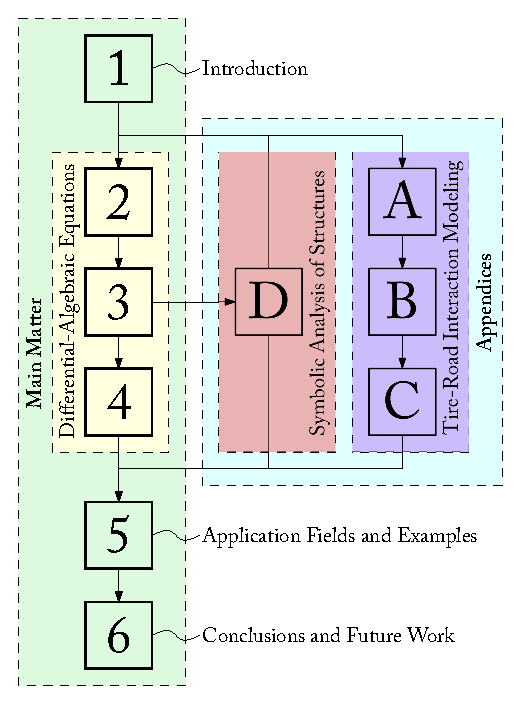
\includegraphics[width=9cm]{./figures/chapter_1/thesis_flowchart}
  \caption{Flowchart of the thesis structure, illustrating the logical progression of the chapters and appendices.}
  \label{chap1:fig:thesis_flowchart}
\end{figure}

% % % % % % % % % % % % % % % % % % % % % % % % % % % % % % % % % % % % % % % %
